\chapter{Data visualization}
\label{cap:studio_data_viz}
\intro{In questo capitolo verrà presentata una panoramica della \gls{datavizg}, spiegandone caratteristiche, usi e principi.
Viene inoltre proposto un metodo di classificazione dei grafici per ottimizzare le visualizzazioni.}\\

\section{Definizione e applicazioni}
\subsection{La necessità di rappresentare i dati}
%INTRO + CAP 1: “Design della mente – infografica e data viz” di Paolo Bottazini, Michele Gotuzzo
La visualizzazione dei dati ha una tradizione millenaria. Sin dagli albori della civiltà umana, 
le persone hanno sviluppato metodi per rappresentare visivamente i dati al fine di renderli più facili da comprendere, 
memorizzare e trasmettere.
Negli ultimi decenni, tuttavia, questa esigenza ha conosciuto un incremento senza precedenti.

Viviamo infatti nell'epoca dell'\gls{infoloadg} e dei \gls{bigdatag}, dove le informazioni
arrivano con una velocità, un volume e una varietà così travolgenti che non siamo in grado di comprenderli se non attraverso
un ulteriore strato di astrazione.
Tale condizione si deve soprattutto allo sviluppo delle tecnologie digitali, grazie alle quali siamo arrivati a disporre di una quantità 
apparentemente infinita di informazioni, tra sapere sociale, motori di ricerca e volontà delle persone di esprimersi.

In questo contesto, la \gls{datavizg} è diventata fondamentale per interpretare e trarre intelligenza da questa grande mole di dati.
Nello specifico, essa consente di fissare l'attenzione in segni maneggevoli - le rappresentazioni grafiche - che consentono una lettura dell'informazione
semplice e intuitiva. Tramite tali segni, è possibile cogliere funzioni strutturali e relazioni impreviste tra fenomeni, oltre che scoprire regolarità tra di essi che 
altrimenti sarebbero rimaste nascoste, facilitando eventuali risoluzioni e valutazioni.

\bigskip
\noindent Possiamo dunque definire la \gls{datavizg} come l'insieme dei meccanismi di traduzione da dati a rappresentazione grafica
mediante i quali l'informazione viene resa più chiara ed efficace. Più precisamente, 
potremmo dire che è un processo atto ad amplificare la cognizione dei dati attraverso
una traslazione di questi in un contesto visivo.


\subsection{Obiettivi della data visualization}
%cap 6: https://onlinelibrary.wiley.com/doi/book/10.1002/9781119209560
Gli obiettivi alla base della \gls{datavizg} sono:
\begin{itemize}
    \item \textbf{Identificare}, ovvero trovare un \emph{dataset} significativo, né troppo banale né troppo complesso, da cui sia possibile
    ricavare delle informazioni utili;
    \item \textbf{Manipolare}, ossia analizzare e combinare i dati in modo da chiarirne il significato;
    \item \textbf{Formattare}, ovvero standardizzare il modo con cui si accede ai dati per una consumazione più efficiente;
    \item \textbf{Presentare}, ossia rappresentare i dati formattati in modo da esprimerne il significato nascosto.
\end{itemize}
\noindent Si desidera dunque massimizzare l'efficacia ed efficienza della visualizzazione. Ciò comporta:
\begin{itemize}
    \item Per quanto riguarda l'efficienza: ridurre la complessità e il rumore nella visualizzazione, eliminando così tutti gli elementi superflui che potrebbero
    portare addirittura a correlazioni incorrette.
    \item Per quanto riguarda l'efficacia: fornire informazioni comprensibili e utili in modo che sia possibile prendere decisioni informate in base a esse.
\end{itemize}

\bigskip
%https://infogram.com/blog/what-is-data-visualization/?_gl=1*1rypyyw*_up*MQ..*_ga*MTg5MzY2NzU2MS4xNzE5MzMxMTgw*_ga_LD50PRQER7*MTcxOTMzMTE3OS4xLjAuMTcxOTMzMTE3OS4wLjAuMA..
\noindent Il fine ultimo di questi obiettivi è quello di:
\begin{itemize}
    \item \textbf{Rendere i dati comprensibili e memorabili},
    \item Facilitare nuove scoperte e \textbf{individuare \emph{trend} e valori anomali},
    \item \textbf{Visualizzare} velocemente \textbf{relazioni e regolarità} nei dati,
    \item \textbf{Rendere più consapevole la presa di decisioni} e stimolare la formulazione di ulteriori domande più specifiche.
\end{itemize} 


\subsection{Applicazioni}
Nell'età contemporanea, il processo di visualizzazione dei dati è ormai diventato essenziale per la gestione quotidiana di qualsiasi 
impresa, governo e organo informativo.

Imprese e pubbliche amministrazioni sfruttano la \gls{datavizg} per comprendere meglio la propria organizzazione e 
prendere decisioni più informate basate sui dati, ad esempio per quanto riguarda la gestione delle risorse e lo sviluppo di strategie future. 
Questo approccio, inoltre, è cruciale anche per la percezione esterna dell'organizzazione e, dunque, per contraddistinguerla da enti a essa analoghi.

Alla stessa maniera, anche per gli organi informativi (e.g. i giornali) la \gls{datavizg} è diventata indispensabile. 
Infatti, solo grazie a essa è possibile ricavare delle intuizioni altrimenti impossibili e rendere fruibili 
tali risultati in maniera chiara e intuitiva. Ciò risulta particolarmente importante per tali organi in quanto la loro \emph{mission} è proprio diffondere 
e comunicare informazioni.



\section{Principi e linee guida}
\subsection{Creare visualizzazioni efficaci}
%https://infogram.com/blog/what-is-data-visualization/?_gl=1*1rypyyw*_up*MQ..*_ga*MTg5MzY2NzU2MS4xNzE5MzMxMTgw*_ga_LD50PRQER7*MTcxOTMzMTE3OS4xLjAuMTcxOTMzMTE3OS4wLjAuMA..
Una buona visualizzazione nasce dall'incontro di comunicazione, \gls{datascienceg} e design.
% immagine da https://venngage.com/templates/diagrams/data-viz-edf4207a-7fb4-47ce-ae1e-df730cc93d78 ma rifatta
\begin{figure}[H] 
    \centering 
    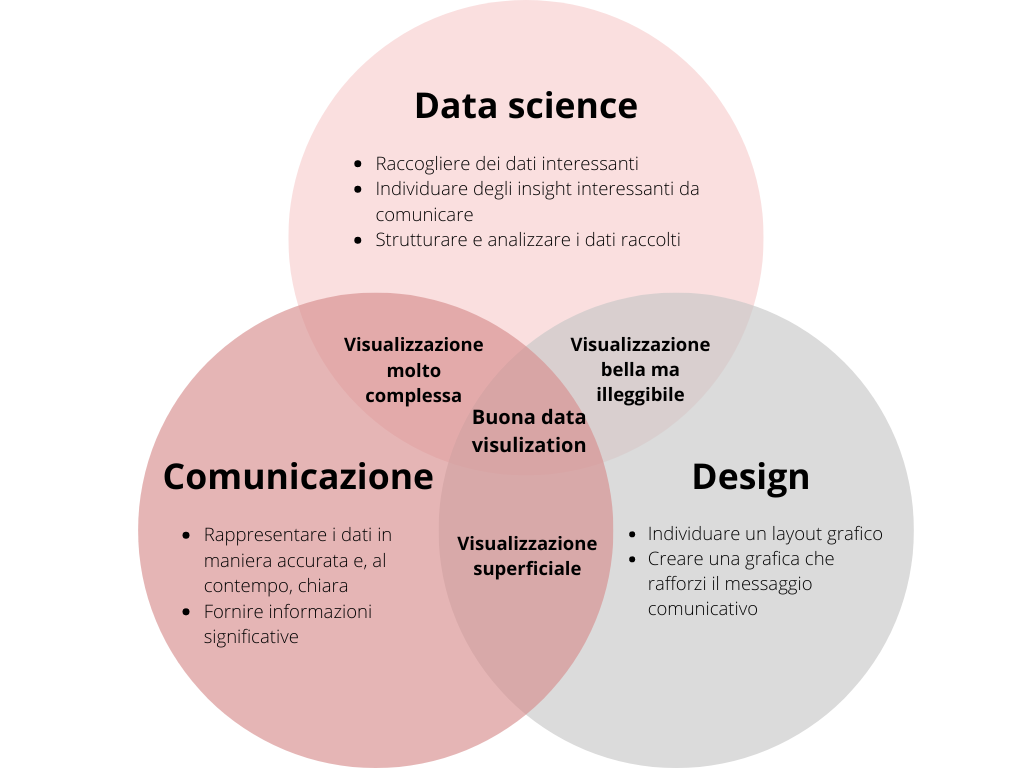
\includegraphics[width=0.8\columnwidth]{data-viz/venn_good_dataviz} 
    \caption{Diagramma di Venn: intersezione tra data science, comunicazione e design nella visualizzazione dei dati}
    \label{fig:venn_good_dataviz}
\end{figure}

\noindent Se realizzata correttamente, infatti, essa è capace di ricavare da \emph{dataset} complessi delle informazioni significative e trasmetterle in maniera intuitiva.
Usando le parole di Edward Tufte, statistico e luminare nel campo della \gls{datavizg}, una visualizzazione dei dati eccellente consiste in
``idee complesse comunicate con chiarezza, precisione ed efficienza''.
% TODO: aggiungere citazione come footnote (%“The visual Display of Quantitative Information” di Edward R. Tufte, CAP 1: Graphical excellence)

%cap1: “L'arte funzionale – Infografica e visualizzazione delle informazioni” di Alberto Cairo
Da ciò ne consegue che l'obiettivo della \gls{datavizg} e ruolo di un architetto dell'informazione è quello di rendere il più efficiente possibile il processo che il cervello
umano compie nell'acquisire conoscenza e saggezza a partire dall'osservazione di fenomeni.
Tale processo può essere descritto, in maniera semplificata, attraverso la cosiddetta gerarchia DIKV (\emph{Data-Information-Knowledge-Wisdom}) di seguito riportata.
\begin{figure}[H] 
    \centering 
    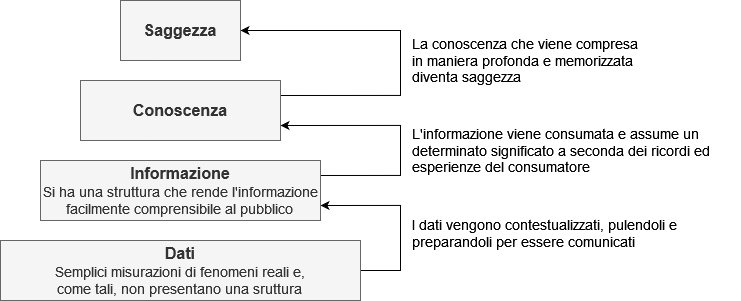
\includegraphics[width=\columnwidth]{data-viz/DIKV} 
    \caption{Gerarchia DIKV}
    \label{fig:DIKV}
\end{figure}

Come si nota subito dall'immagine \ref{fig:DIKV}, è essenziale ottenere dati puliti, completi e rappresentativi (responsabilità della \gls{datascienceg}). Solo successivamente sarà possibile rappresentare tali dati e 
ottenere una conoscenza valida (responsabilità di comunicazione e design).

\bigskip
%“L'arte funzionale – Infografica e visualizzazione delle informazioni” di Alberto Cairo
% cap 2
\noindent Nella visualizzazione dei dati in sé, bisogna tener conto innanzitutto che la forma grafica delle informazioni non è di per sé un'applicazione artistica; infatti, 
essa deve anche coadiuvare il fruitore in attività intellettive. Pertanto, la forma deve aspirare a oggettività, precisione e, soprattutto, funzionalità.
Per descrivere tale principio, possiamo dunque prendere in prestito le parole di Louis Sullivan sull'architettura modernista del XX secolo: ``La forma segue la funzione''. 
Tale massima può infatti essere applicata anche all'architettura dell'informazione nel contesto della \gls{datavizg}, giacché
un complesso di dati può assumere più forme, ma non tutte le forme sono sempre adatte e usabili. Infatti, la loro scelta deve dipendere dal
tipo di dati e obiettivo della rappresentazione. Ne consegue che più preciso è lo scopo, più limitata sarà la gamma di forme tra cui scegliere.

Il processo di decisione della rappresentazione grafica viene meglio approfondito nella sezione \ref{sec:classificare_grafici}.

\bigskip
\noindent Una volta decisa la forma migliore, bisogna comunque adattarla alla visualizzazione del caso specifico attraverso delle scelte di design.
In tal senso, si può adottare un approccio più minimalistico, promosso dal sopracitato Edward Tufte, o un approccio più ``artistico'', 
sostenuto da Nigel Holmes, famoso grafico specializzato nel design delle informazioni.

%“The visual Display of Quantitative Information” di Edward R. Tufte
%CAP 1: Graphical excellence
Per Tufte è essenziale combinare una semplicità di design a complessità dei dati. Per lui, il fruitore della visualizzazione deve poter ricavare il maggior numero di idee e informazioni dal minor uso possibile di spazio e inchiostro.
A tal proposito, egli sviluppa le seguenti formule: 
\begin{center}
    $\text{Rapporto dati-inchiostro} = \frac{\text{inchiostro usato per la codifica dei dati}}{\text{inchiostro totale usato per la stampa del grafico}}$
\end{center}
\begin{center}
    $\text{Densità dei dati} = \frac{\text{numero di voci in una matrice di dati}}{\text{area occupata dal grafico}}$            %CAP 8: Data density and small multiples
\end{center}
% TODO: aggiungere footnote che questa parte si intende solo quella dei datiDensità = number entries in una matrice di dati / area del grafico.
%Meglio se è più alta (mappe è altissima), risulta anche essere più affidabile. Bisogna comunque evitare di sovrappopolare lo spazio, in quel caso conviene utilizzare tecniche di data-reduction (averaging, clustering, smoothing).
%Attenzione! Stiamo parlando della parte di dati, per quanto riguarda la parte non strettamente riguardante questi (chartjunk) meglio meno.
evidenziando che più il rapporto è alto, migliore è la rappresentazione. Ciò implica che sia necessario evitare di utilizzare tutti gli elementi decorativi o, più in generale, tutte le parti che possono essere omesse 
senza perdere dati, ovvero tutto ciò che Tufte chiama \gls{chartjunkg} (e.g. la maggior parte delle griglie e sfondi posti sotto i grafici).

%“L'arte funzionale – Infografica e visualizzazione delle informazioni” di Alberto Cairo
%cap 3
D'altra parte, Holmes sostiene che ci si può divertire con la forma, purché la funzione principale rimanga comunicare i dati. Infatti, ciò che Tufte potrebbe considerare \gls{chartjunkg}, e dunque superfluo,
potrebbe invece rivelarsi utile al processo di memorizzazione e dunque portare più facilmente alla saggezza. 

%“L'arte funzionale – Infografica e visualizzazione delle informazioni” di Alberto Cairo
%Cap 4
Qualsiasi approccio si decida di intraprendere, rimane comunque essenziale sfruttare lo spazio a disposizione per ricercare la profondità, seppur rimanendo nei limiti dettati dal tipo di fruitori.
Tale profondità si concretizza quasi sempre tramite la rappresentazione di dati multivariati, che consentono l'analisi di un fenomeno in maniera più accurata. %multivariato da %“The visual Display of Quantitative Information” di Edward R. Tufte, CAP 1: Graphical excellence
Le informazioni non devono infatti essere semplificate o snellite dalla visualizzazione, bensì devono essere solamente chiarite. La rappresentazione dovrebbe permettere dunque di suscitare riflessioni non superficiali ed evidenziare tendenze, \emph{pattern} 
o fenomeni altrimenti invisibili. 
Solo in un secondo momento ci si può dedicare all'estetica della presentazione, utilizzando gli spazi rimanenti. Tale precauzione è da prendere affinché i dati ricevano subito tutto lo spazio necessario ed eventuali
effetti speciali o decorazioni siano inseriti solo se se ne presenta l'opportunità.


\subsection{Linee guida}
%“The visual Display of Quantitative Information” di Edward R. Tufte
%CAP 1: Graphical Integrity
Nel visualizzare dati è necessario garantire che le informazioni siano rappresentate accuratamente e senza distorsioni.
A tal scopo, è dunque necessario perseguire un'\textbf{integrità grafica}. Ciò implica l'uso di:
\begin{itemize}
    \item proporzioni corrette tra la rappresentazione dei numeri sul grafico e le quantità numeriche fornite, come pure tra il 
    numero di dimensioni rappresentate graficamente e il numero delle variabili nei dati;
    \item scale appropriate che mostrino la vera variazione dei dati (e.g. scale con intervalli regolari);
    \item etichette dettagliate e chiare che non fuorviino l'utente;
    \item elementi che contestualizzino il grafico.
\end{itemize}

%“The visual Display of Quantitative Information” di Edward R. Tufte
%CAP 9: AESTHETICS AND TECHNIQUE IN DATA GRAPHICAL DESIGN
\noindent Come accennato precedentemente, altrettanto importante è la \textbf{scelta del design}. Ciò include:
\begin{itemize}
    \item La scelta di un formato e \emph{layout} appropriato, scegliendo la combinazione di frasi, tabelle
    e grafici che meglio mostri la riflessione che si vuole comunicare (e.g. per più di due numeri, conviene usare una tabella piuttosto che una frase). Ciò comporta:
    \begin{itemize}
        \item per l'occidente, un orientamento (specie per quanto riguarda il testo) che va dall'alto a sinistra verso il basso a destra;
        \item l'uso di grafici corredati da piccoli messaggi di chiarimento, piuttosto che spiegazioni sparse.
    \end{itemize}
    \item L'uso simbiotico, coerente e diretto di parole, numeri e figure.
    \item Visualizzare i dati in maniera accessibile, anche e soprattutto per quanto riguarda dettagli di dati complessi. Ciò comporta:
    \begin{itemize}
        \item l'uso di codifiche non troppo elaborate, che non necessitino il continuo controllo della legenda;
        \item tenere in considerazione anche le persone daltoniche e \emph{color-deficient} nella scelta dei colori del grafico (se presenti);
        \item l'uso di caratteri leggibili.
    \end{itemize}
\end{itemize}



\section{Classificare i grafici}\label{sec:classificare_grafici}
Lo sviluppo e disponibilità al pubblico di nuovi strumenti avanzati ha consentito anche a utenti non esperti di visualizzare dati ed estrarne informazioni dettagliate, 
permettendo loro di creare grafici e diagrammi.
Tuttavia, persiste ancora un ampio divario di conoscenza tra questi utenti e i modelli visivi esistenti.
Ne consegue che spesso le forme visive scelte per la rappresentazione non sono le più efficaci essendo limitate da un ristretto numero di opzioni conosciute.
In alcuni casi, addirittura, la rappresentazione scelta risulta essere anche poco comprensibile o fuorviante per il caso d'uso specifico.

Senza una classificazione chiara, diventa dunque difficile per questo tipo di utenti selezionare la tecnica di visualizzazione più adeguata.
Nelle seguenti sezioni, si esaminano dunque dei criteri di classificazione identificati, assieme a uno strumento prototipale che mira ad 
automatizzare questo processo di classificazione.


\subsection{Metodo di classificazione}
I criteri principali da tenere in considerazione nella scelta del grafico sono:
\begin{itemize}
    \item l'obiettivo della visualizzazione,
    \item i tipi di dati disponibili.
\end{itemize}

\subsubsection{Obiettivi della visualizzazione}\label{subsubsec:obj}
Quando parliamo di ``obiettivo della visualizzazione'' intendiamo il tipo di relazione tra i dati che vogliamo mettere in evidenza attraverso
la rappresentazione grafica. I principali obiettivi individuati sono:
\begin{enumerate}
    \item \textbf{Divergenza}, quando si vogliono mettere in luce le differenze di valori a partire da un punto fisso (solitamente lo 0, ma può essere
    ad esempio anche una media).
    \begin{itemize}
        \item Esempio: confrontare la produttività del turno di giorno con quello del turno di notte.
    \end{itemize}
    \item \textbf{Correlazione}, quando si vuole enfatizzare la relazione tra due o più variabili. In questi casi, il fruitore della visualizzazione assumerà che le 
    variabili coinvolte siano in relazione causale, pertanto se così non fosse è necessario specificarlo.
    \begin{itemize}
        \item Esempio: esplorare come la qualità del sonno influenzi le prestazioni accademiche.
    \end{itemize}
    \item \textbf{\emph{Ranking}}, quando si vuole mostrare la posizione degli elementi rispetto agli altri e il loro valore effettivo passa in secondo piano.
    \begin{itemize}
        \item Esempio: mostrare i dieci paesi con il tasso di inquinamento più alto.
    \end{itemize}
    \item \textbf{Distribuzione}, quando si vogliono mostrare eventuali \emph{pattern} nei dati, evidenziando valori ed eventi di un \emph{dataset} e per quali casi essi si verificano. 
    \begin{itemize}
        \item Esempio: mostrare la frequenza di incidenti stradali per tipo di veicolo.
    \end{itemize}
    \item \textbf{Cambiamento nel tempo}, quando si vogliono enfatizzare dei \emph{trend} che variano nel tempo.
    \begin{itemize}
        \item Esempio: analizzare come l'uso dei social media è cambiato negli ultimi cinque anni.
    \end{itemize}
    \item \textbf{Composizione}, quando si vuole mostrare come una singola entità viene suddivisa nelle sue componenti.
    \begin{itemize}
        \item Esempio: mostrare la composizione delle emissioni di gas serra per settore industriale.
    \end{itemize}
    \item \textbf{Grandezze}, quando si vogliono comparare grandezze, che siano esse assolute (per un maggior livello di dettaglio) o relative. 
    \begin{itemize}
        \item Esempio: mostrare la dimensione del mercato degli smartphone in termini di volumi di vendita.
    \end{itemize}
    \item \textbf{Spazi}, quando si vogliono mostrare \emph{pattern} geografici o posizioni precise.
    \begin{itemize}
        \item Esempio: mostrare i paesi con la maggiore concentrazione di risorse naturali.
    \end{itemize}
    \item \textbf{Flussi}, quando si vogliono mostrare volumi o intensità del movimento/cambiamento tra due o più stati o condizioni.
    \begin{itemize}
        \item Esempio: esplorare la rete di interconnessioni finanziarie tra le banche.
    \end{itemize}
\end{enumerate}

\subsubsection{Tipi di dati}
Una prima distinzione nel tipo di dati riguarda:
\begin{itemize}
    \item \textbf{dati numerici},
    \item \textbf{dati categorici}.
\end{itemize}
Il \emph{dataset} fornito per la visualizzazione potrà dunque essere composto da dati tutti numerici, tutti categorici oppure da un mix dei due.

\bigskip
\noindent Un'altra distinzione si ha tra:
\begin{itemize}
    \item \textbf{dati univariati}, quando ho un \emph{dataset} molto piccolo composto da una sola variabile;
    \item \textbf{dati multivariati}, quando ho un \emph{dataset} composto da più variabili.
\end{itemize}

\bigskip
\noindent In base alle suddette classificazioni, si può specificare ulteriormente il tipo di dato:
\begin{itemize}
    \item In caso di \emph{dataset} con multiple variabili numeriche:
    \begin{itemize}
        \item \textbf{dati ordinati}, dove è presenta almeno una variabile numerica che è ordinata;
        \item \textbf{dati non ordinati}, dove l'ordine non è rilevante.
    \end{itemize}
    \item In caso di \emph{dataset} con multiple variabili categoriche:
    \begin{itemize}
        \item \textbf{organizzazione in sottogruppi}, una o più variabili categoriche specificano e rappresentano una sottopopolazione di un'altra variabile categorica;
        \item \textbf{organizzazione indipendente}, le variabili categoriche sono indipendenti tra di loro;
        \item \textbf{organizzazione gerarchica}, una o più variabili categoriche specificano un rapporto gerarchico rispetto ad un'altra variabile categorica padre.
    \end{itemize}
    \item In caso di almeno una variabile numerica e una categorica, con multiple variabili categoriche solo se organizzate in sottogruppi o in relazione gerarchica:
    \begin{itemize}
        \item \textbf{Una singola occorrenza}, quando a ogni individuo della popolazione, individuato dalle variabili categoriche, corrisponde un solo dato numerico;
        \item \textbf{Multiple occorrenze}, quando a ogni individuo della popolazione, individuato dalle variabili categoriche, corrispondono multipli valori numerici.
    \end{itemize}
\end{itemize}


\subsection{Chart-chooser}
%file criteri_scelta_grafico_v0.1.0 + codice + prompt LLM
%fonte: https://www.data-to-viz.com/ e https://ft-interactive.github.io/visual-vocabulary/
\emph{Chart-chooser} è uno strumento prototipale sviluppato nel corso dello stage che si serve del metodo di classificazione descritto 
nelle pagine precedenti per consigliare a un utente non esperto uno o più grafici che potrebbero rappresentare al meglio i dati disponibili.
Tale compito di classificazione viene gestito e realizzato principalmente tramite un \gls{sistemadiregoleg}, il cui funzionamento viene approfondito al paragrafo
\hyperref[subsubsec:rules]{Implementazione del sistema di regole}.

Lo strumento è disponibile a \href{http://www.overleaf.com}{questo link}.
% TODO: inserire link github 

\subsubsection{Analisi dei dati}
In primis, è necessario individuare il numero di variabili numeriche e categoriche presenti nel \emph{dataset}.
\emph{Chart-chooser} effettua tale processo in maniera semplificata, controllando se il primo valore per ogni variabile
è un numero (variabile numerica) o una stringa (variabile categorica).

Nel caso sia necessario, viene inoltre richiesto all'utente di rispondere ad alcune domande per chiarire ulteriori aspetti riguardanti il tipo 
di dato e individuare le ulteriori sotto-distinzioni (come descritte nella sezione precedente). Ad esempio, nel caso si abbiano dati multivariati numerici verrà chiesto 
se i dati sono ordinati o meno, mentre se si hanno dati univariati numerici non saranno necessarie ulteriori domande.

\subsubsection{Individuazione dell'obiettivo}
Una volta definito il tipo di dato è necessario individuare l'obiettivo della visualizzazione.
A tal fine, \emph{Chart-chooser} richiede all'utente di fornire una breve descrizione di ciò che vuole rappresentare e comunicare.
Il testo immesso viene poi elaborato da un \gls{llm}, il quale interpreta la descrizione e ne estrae l'obiettivo più pertinente tra i nove possibili (definiti e descritti in \ref{subsubsec:obj}). 
Come \gls{llm} viene utilizzato \textbf{\gls{llama7bg}} attraverso \textbf{\gls{llamacppg}}, reso disponibile dall'azienda ospitante. I parametri sono perlopiù quelli di default, tranne la temperatura che viene 
impostata a 0 per garantire che l'output del modello sia il più predicibile possibile e restituisca solamente il numero dell'obiettivo.

\bigskip
\noindent Per quanto riguarda invece il metodo di \gls{promptengg} utilizzato, si adopera una tecnica di \gls{fsl} implementata nello scenario dell'\gls{icl}.
Nello specifico, per ogni obiettivo vengono fornite al \gls{llm} alcune descrizioni d'esempio in modo tale da facilitare al modello il compito di classificazione e migliorarne le
prestazioni. Questo approccio permette al \gls{llm} di comprendere meglio il contesto e rispondere con una maggiore precisione.

Il prompt utilizzato è il seguente:
\begin{lstlisting}[style=htmlcssjs]
This is a conversation between User and Llama, a friendly chatbot. Llama is helpful, kind, honest, good at writing, and never fails to answer any requests immediately and with precision.

User: 
Dati i seguenti obiettivi:
Obiettivo 1: Mostrami la differenza tra i dati; Confronta due serie di dati divergenti; Mostrami la variazione rispetto a un valore.
Obiettivo 2: Mostrami un dato in relazione ad un altro; Mostrami come sono associati i due dati; Mostrami la correlazione tra un dato e i suoi due fattori.
Obiettivo 3: Mostrami la classifica; Mostrami i top; Mostrami i dati più importanti; Mostrami i più comuni; Mostrami i principali.
Obiettivo 4: Mostrami quante volte si verifica un evento; Mostrami la distribuzione del dato; Mostrami la media; Mostrami la frequenza.
Obiettivo 5: Mostrami la variazione nel tempo del dato; Mostrami la tendenza del dato nel tempo; Mostrami le differenze tra i dati nel tempo; Mostrami il cambiamento dei dati nel tempo; Mostrami le previsioni future.
Obiettivo 6: Mostrami i componenti del dato; Mostrami il dato diviso nei sottogruppi; Mostrami la struttura del dato; Mostrami la ripartizione del dato.
Obiettivo 7: Mostrami la dimensione effettiva del dato; Mostrami le unità; Mostrami la misura del dato; Mostra la rilevanza del dato all'interno di un contesto; Mostrami la grandezza dei dati.
Obiettivo 8: Mostrami la posizione; Mostrami i flussi nel mondo; Mostrami la mappa di distribuzione; Mostrami i paesi in cui si verifica l'evento; Mostrami la variazione nello spazio del dato.
Obiettivo 9: Mostrami i flussi tra i vari punti; Mostrami la rete; Mostrami le relazioni e la loro intensità; Mostrami cosa influisce nel dato; Mostrami come sono relazionati all'interno di un sistema. 

Classifica la seguente frase, dimmi solamente il numero dell'obiettivo senza altre parole: 
${descrizione_utente}
Llama:
\end{lstlisting}
% TODO: rivedere prompt su chart-chooser e inserire modello usato corretto (7b?)

\subsubsection{Implementazione del sistema di regole}\label{subsubsec:rules}
Le informazioni raccolte sono utilizzate da un \gls{motoreregoleg} per combinare le analisi e le classificazioni effettuate e restituire il nome dei possibili grafici applicabili al caso d'uso, se presenti.
Si precisa, infatti, che non per tutti gli obiettivi sono presenti tutti i tipi di dato. Pertanto, la combinazione potrebbe portare a un risultato nullo.

Il \gls{motoreregoleg} scelto è \textbf{\gls{jsonrulesg}}. Tale decisione è motivata dalla sua leggerezza e velocità, nonché dal fatto che le regole siano semplici strutture \gls{jsong}, 
il che le rende più leggibili dall'uomo e facili da mantenere.

\bigskip
\noindent Gli elementi principali che caratterizzano tale sistema sono:
\begin{itemize}
    \item I \emph{fatti}, ovvero dei valori costanti o funzioni pure.
    \item Le \emph{regole}, ovvero delle strutture composte da:
    \begin{itemize}
        \item \emph{Condizioni}, nella forma \texttt{[fact: nome\_fatto, operator: tipo\_operatore, value: valore\_da\_controllare]}
        che rappresentano i ``requisiti'' della regola, soddisfatti se la relazione definita dall'operatore tra il valore del \emph{fatto} e il valore prestabilito 
        indicato risulta vera. Si precisa, inoltre, che possono essere creati insiemi di queste \emph{condizioni} attraverso l'uso di operatori booleani.
        \item \emph{Eventi}, ovvero delle operazioni che il \emph{motore} esegue in base al soddisfacimento o meno delle \emph{condizioni}. 
    \end{itemize}
    \item Il \emph{motore di inferenza} in sé, a cui vengono dati in input i \emph{fatti} e aggiunte le \emph{regole}. Esso è il cuore del \gls{motoreregoleg} in quanto si occupa di valutare
    le \emph{regole} basandosi sui \emph{fatti} forniti, innescando \emph{eventi} a seguito del soddisfacimento o meno delle \emph{condizioni}.
\end{itemize}
%TODO: inserire codice esempio cose

\bigskip
\noindent Per quanto riguarda il funzionamento specifico di ``Chart-chooser'', si hanno come \emph{fatti} iniziali solamente il numero di variabili numeriche e categoriche. 
Per quanto riguarda gli altri \emph{fatti}, che richiedono un input da parte dell'utente (e.g. l'obiettivo o il fatto di essere dati numerici ordinati o meno), questi sono 
forniti al \emph{motore} durante la sua esecuzione, all'innescarsi di determinati \emph{eventi}. 
Ciò permette di poter valutare subito le regole sui \emph{fatti} già noti e nel frattempo poter ottenere dall'utente il valore dei rimanenti, fermando eventualmente l'esecuzione del \emph{motore} solo
prima di regole che necessitano dei \emph{fatti} ancora sconosciuti. % TODO: ottenere come promise?
In tale maniera, inoltre, vengono richiesti all'utente e forniti al \emph{motore} solamente i \emph{fatti} che concernono la situazione specifica. Ad esempio, nel caso in cui si abbiano solamente dati numerici, 
non verrà chiesta all'utente e non sarà fornita inutilmente al \emph{motore} l'informazione riguardante l'organizzazione delle variabili categoriche.

Il funzionamento descritto è reso possibile grazie all'adozione di un \gls{sistemadiregoleg} gerarchico. Nello specifico, a ciascuna \emph{regola} viene attribuita una \emph{priorità} che ne determina l'ordine di valutazione:
una \emph{priorità} maggiore comporta una valutazione anticipata; mentre, in caso di più \emph{regole} ad uguale \emph{priorità}, queste verranno valutate in parallelo.
Questo meccanismo viene sfruttato per realizzare una classificazione stratificata, in cui ogni livello di \emph{priorità} rappresenta una fase di classificazione più dettagliata rispetto al livello precedente. 
Ne consegue che le \emph{regole} appartenenti allo stesso livello siano mutualmente esclusive, poiché ciascuna di esse definisce un gruppo specifico in cui possono essere catalogati i dati forniti.
Per consentire ai livelli inferiori di conoscere il gruppo identificato precedentemente e procedere con ulteriori sottoclassificazioni dello stesso, viene aggiunto ai \emph{fatti} un valore booleano per ogni \emph{regola}. 
Tale valore rappresenta il soddisfacimento delle \emph{condizioni} della \emph{regola}, assumendo il valore di \texttt{true} in caso positivo o \texttt{false} altrimenti.

\bigskip
\noindent Si ha dunque il seguente \gls{sistemadiregoleg}:

\begin{figure}[H] 
    \centering 
    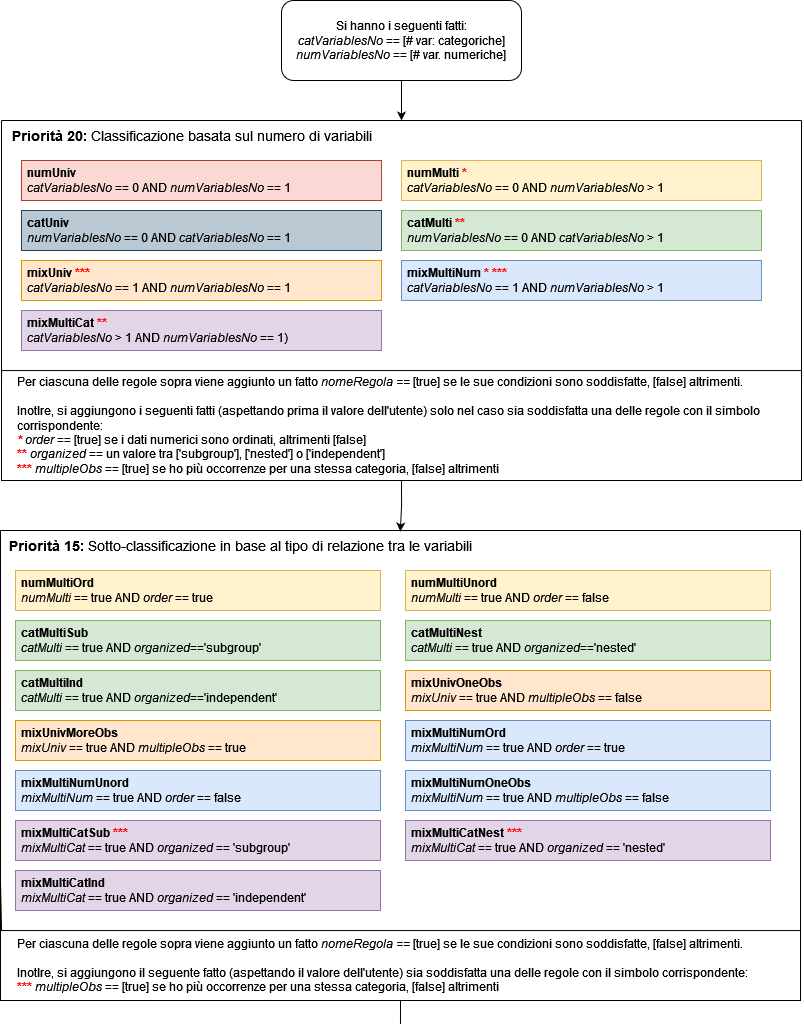
\includegraphics[width=\columnwidth]{data-viz/rules_pt1} 
    \caption{Sistema gerarchico di priorità per le regole di \emph{Chart-chooser} - priorità 20 e 15}
    \label{fig:rules_pt1}
\end{figure}
\begin{figure}[H] 
    \centering 
    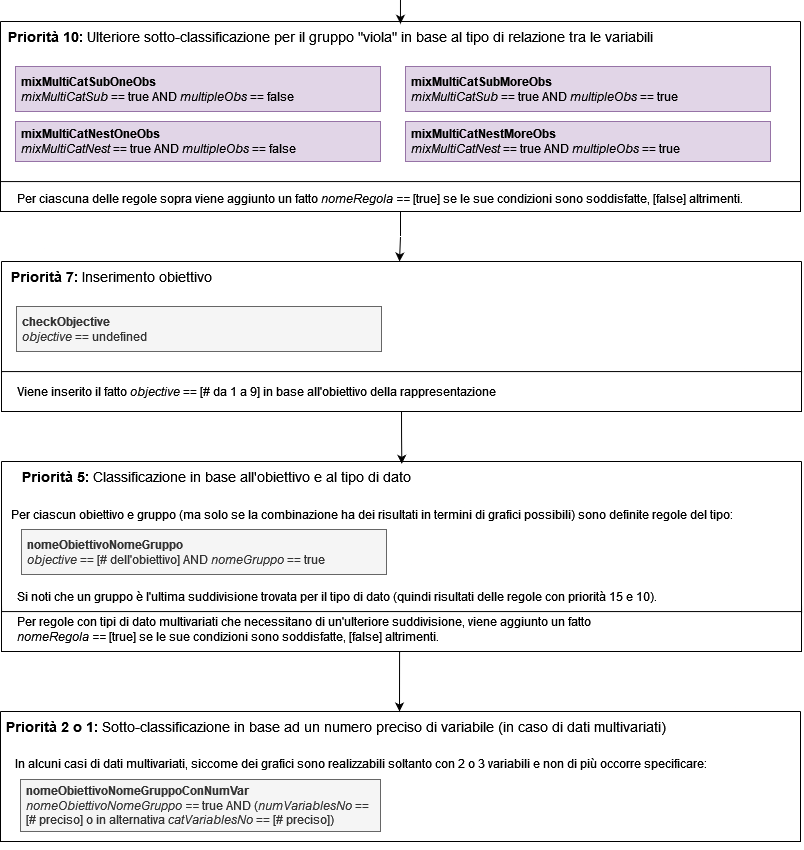
\includegraphics[width=\columnwidth]{data-viz/rules_pt2} 
    \caption{Sistema gerarchico di priorità per le regole di \emph{Chart-chooser} - priorità dalla 10 all'1}
    \label{fig:rules_pt2}
\end{figure}

Dalla figura \ref{fig:rules_pt2} si osserva un'eccezione rispetto al funzionamento descritto in precedenza per quanto riguarda il livello di \emph{priorità} 7. In questo caso, il livello non effettua alcuna suddivisione, 
bensì si occupa solamente di recuperare il numero di obiettivo, necessario per poter proseguire con la classificazione. Tale configurazione permette di valutare le \emph{regole} relative al tipo di dato mentre  
il numero di obiettivo viene ricavato dall'elaborazione del \gls{llm} dell'input utente, anziché attendere passivamente il completamento di quest'ultima.


\subsubsection{Proposta di grafici}
Le \emph{regole} di \emph{priorità} minore o uguale a 5, se soddisfatte, innescano degli \emph{eventi} che hanno come parametri il nome dei grafici adatti al caso d'uso specifico indicato dalla classificazione fornita dalla \emph{regola} stessa. 
Il \emph{motore}, dunque, al termine della valutazione delle \emph {regole}, controlla gli \emph{eventi} emessi e mostra all'utente i parametri di questi, ovvero il nome dei grafici trovati (se presenti).

%Dopo un attento studio dei grafici e metodi di classificazioni trovati.
%TODO inserire fonti? tecnologie usate js?


\subsubsection{Limitazioni dello strumento}
Come già accennato precedente \emph{Chart-chooser} è uno strumento prototipale, presenta infatti diverse limitazioni.
Innanzitutto, l'applicativo è disponibile soltanto da riga di comando e non dispone di un'interfaccia grafica.
Inoltre, esso richiede che i dati siano disponibili in locale e che siano formattati secondo uno schema specifico
(una specifica struttura \gls{jsong}). 
L'utente deve, altresì, essere a conoscenza del \emph{dataset} per poter rispondere correttamente alle domande relative ad esso.

Ciononostante, \emph{Chart-chooser} ha il potenziale per essere migliorato e offrire un'esperienza utente più semplice e intuitiva. 
Una possibile direzione per uno sviluppo futuro potrebbe essere l'implementazione di un \emph{parsing} automatico dei dati e la capacità di 
rilevare e interpretare informazioni chiave direttamente dai \emph{dataset}, riducendo così la dipendenza dall'intervento dell'utente. 